
Let
\begin{align}
    \Vec{A}=\myvec{-3\\-4}
\end{align}
\begin{align}
    \Vec{B}=\myvec{-8\\7}
\end{align}
\begin{enumerate}
\item Using section formula for internal division, 
\begin{align}
\vec{S}&=\large{\frac{7\myvec{-8\\7}+5\myvec{-3\\-4}}{\brak{7+5}}}   
\\
&=\frac{1}{12}\myvec{{-71} \\ {29}}
\end{align}
\item Similarly, for external division, 
\begin{align}
\vec{S}&=\large{\frac{7\myvec{-8\\7}-5\myvec{-3\\-4}}{\brak{7-5}}}   
&=\frac{1}{2} \myvec{{-41} \\ {69}}
\end{align}

Fig. \ref{1/18fig} plots the desired points.
\begin{figure}[!ht]
\centering
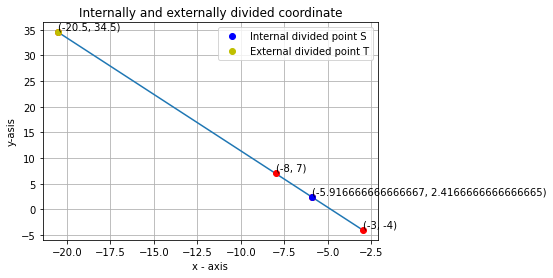
\includegraphics[width=\columnwidth]{solutions/1/18/Internal and external point.png}
\caption{ Plot of coordinate of the point which divides internally and externally }
\label{1/18fig}
\end{figure}
 \end{enumerate} 
